\chapter{Methodology Overview}
\label{sec:methodology}
\section{Introduction}
To answer the research questions and test the hypotheses proposed in chapter \ref{introduction}, a following methodology with 3 steps is employed:
\begin{enumerate}
\item Accented speech recordings collection. The very first step is to have accented speech data. Then, the accentedness score of each accented speaker needs to be collected to quantify how strong the foreign accent is for native L2 speakers.
\item Measurements related to perceived accentness will be extracted from the acoustic signal.This involves different feature extraction schemes because some measurements represent pronunciation characteristics and some represent prosodic characteristics. This study will extract measurements related to both L1 and L2.
\item Statistical data analysis is to examine how the perceived accentedness scores are decided by those independent variables extracted from the acoustic signal. It includes correlational analysis between signal independent variable and accentedness scores and regression analysis between groups of independent variables and accentedness scores. This study will do regression analyses with different groups of independent variables, for example group of independent variables that are only related to L2 and group of independent variables that are related to both L1 and L2.
\end{enumerate}
This chapter will mainly focus on the first two parts and following chapters will introduce the details of data analysis and corresponding results. Part of this chapter is excerpted from a conference paper by the author \citep{tu2018investigating}.

\section{Data collection}

\subsection{Dataset selection}

Many non-native speech datasets have been published in the literature \citep{raab2007non}. However, most of them are either not publicly available nor do not have speakers from several different L1s. To have more control on the datasets, the GMU speech accent archive (SAA) \cite{weinberger2013speech} was chosen as the data source of the speech recordings used in this dissertation. The SAA provides speech samples by speakers from over 300 different L1s. More than 2000 speakers (there are 600 native English speakers currently) read the same paragraph in English:

\vspace{4pt}
\textit{Please call Stella.  Ask her to bring these things with her from the store:  Six spoons of fresh snow peas, five thick slabs of blue cheese, and maybe a snack for her brother Bob.  We also need a small plastic snake and a big toy frog for the kids.  She can scoop these things into three red bags, and we will go meet her Wednesday at the train station.}
\vspace{4pt}

This paragraph was chosen because it includes all of the phonological features considered part of native English speech \citep{kunath2010wisdom}. With transcription available, it is also easy to derive fine-grained measurements on small phonological unit with computed start and end time. SAA also provides detailed information of the speaker, including age, gender, birth place, native language, English residence country, length of residence and age of English onset. The non-native speech corpus used in this study is a subset of the GMU SAA. Four foreign languages: German (9 females, 21 males), French (15 females, 15 males), Mandarin (15 females, 15 males) and Spanish (15 females, 15 males), each of which has 30 speakers. 30 native English speakers (15 females, 15 males) were also added to the set as native speakers. Those four foreign languages are selected because their distances to English in phonetic and prosodic subspace are different. The English residence country was limited to the USA and native English speakers were also born in the USA. This resulted in 150 speakers in the final dataset. The length of each speaker's recording varies in a range from 15-40 seconds. The sampling rate was reduced to 16kHz from 44kHz.



\subsection{Accentedness score collection}

SAA does not provide accentedness scores for their speech recordings. In order to quantify the perceived accentedness score , the best way is to ask native speakers of American English to rate the foreign speakers in the dataset. Considering the time and money cost of on-site data collection, Amazon Mechanical Turk (AMT), which is the most popular online crowdsourcing platform, will be chose to acquire the accentedness score from multiple native American English speakers. The study by \cite{kunath2010wisdom} also collect accentedness score for recordings from SAA on AMT and they reported that the collected ratings were reliable enough.

The first step of the accentedness score collection is to find annotators to participate in the task and design the accentedness score scale. The current accentedness annotation task has several requirements for the annotators: 1) Born in the USA (Must be native speaker of American English) 2) Monolingual (Only speak American English) 3) Don't speak the four target foreign languages (Further make sure they do not speak any of the four foreign languages). 4) No hearing impairment (Make sure they can perceive the foreign accent). 5) At least finished 10 HITs that are approved (Make sure they have experience using the AMT). 6) Human Intelligence Task (HIT)\footnote{The annotation task on AMT is called HIT.} approval rate is over 90\% on AMT (Make sure they devote themselves in each annotation task). Only qualified raters are allowed to do the annotation. To discretize the accentedness, this study employs a four-point scale where one represents no accent/negligible accent, two represents mild accent, three represents strong accent, and four represents very strong accent. This scale has been used in previous collected datasets for example the CSLU: Foreign Accented English datasets \citep{choueiter2008empirical} and it is believed that for non-expert annotators a 4-point scale is of less amount of annotation work and higher accuracy compared to a larger scale.

AMT needs an annotation protocol that clearly introduces the whole procedure to finish the annotation task. A website was designed to realize this protocol. The diagram in figure \ref{fig:amt_procedure} shows the whole procedure of the data annotation process.

\begin{figure}[t]
\centering
\captionsetup{justification=centering}
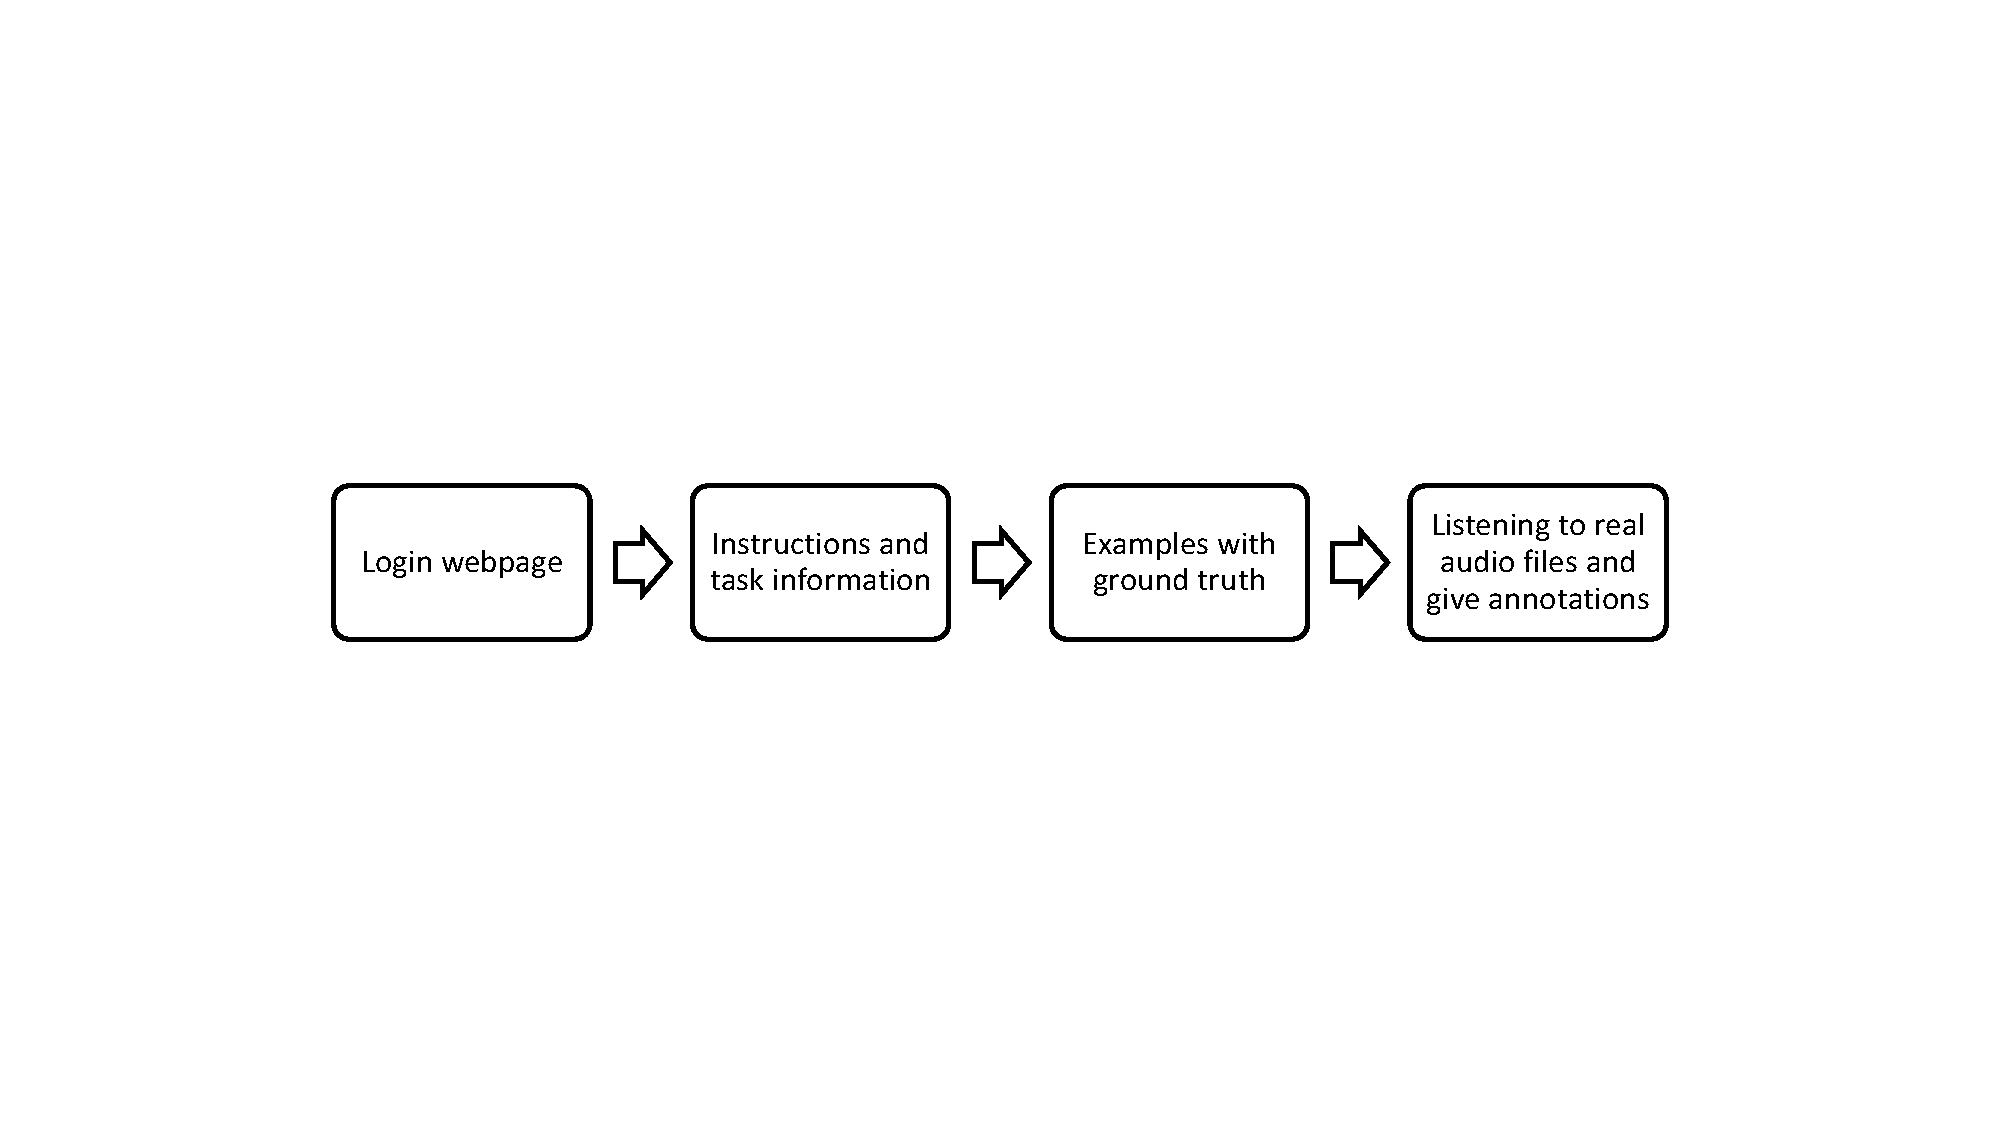
\includegraphics[width = 1.0\linewidth]{figures/amt_procedure.pdf}
\caption{The four steps of the annotation webpage.}
\label{fig:amt_procedure}
\end{figure}

\begin{enumerate}
\item The annotators will first see a webpage (as shown in figure \ref{fig:amt_login}) asking them to create a new user or login as a return user. The user ID will be used as identifier to locate their ratings.
\item After finishing step 1, a detailed task instruction and information will be shown to the annotators. The detail is in appendix \ref{sec:appendix1}. There is also a consent form (in appendix \ref{sec:appendix2}) for the annotators.
\item Then, four recordings, which are with no accent, mild accent, strong accent and very strong accent respectively, are presented to the annotators for them to get familarization with the 4-point rating scale, as shown in figure \ref{fig:amt_example}. The groundtruth labels are provided by native American English speakers.
\item At last, annotators move to the real listening task, as shown in figure \ref{fig:amt_listen}. Each annotator first listen to the recording and make a choice about the degree of perceived foreign accent and whether the annotator is confident in the response. All 150 speech recordings (including native English speech and accented speech) are randomly permuted in order. If we ask the workers on AMT to listen all of the utterances, the task will take more than 1 hour and a lot of factors will impact the quality of the collected ratings, such as worker's fatigue \citep{rzeszotarski2013inserting}. To avoid this, all the utterances are segmented to take just the first 10 seconds, resulting in 25 minutes listening time for each worker. Previous study \citep{munro1995foreign} has shown that the sentence length in the range of 7-13 seconds has little impact on the perceived accentedness. Considering the annotation time and a 2 minutes break, each worker needs to spend about 30-40 minutes for this task. Those annotators finish the task will be rewarded \$1.5.
\end{enumerate}


\begin{figure}[t]
\centering
\captionsetup{justification=centering}
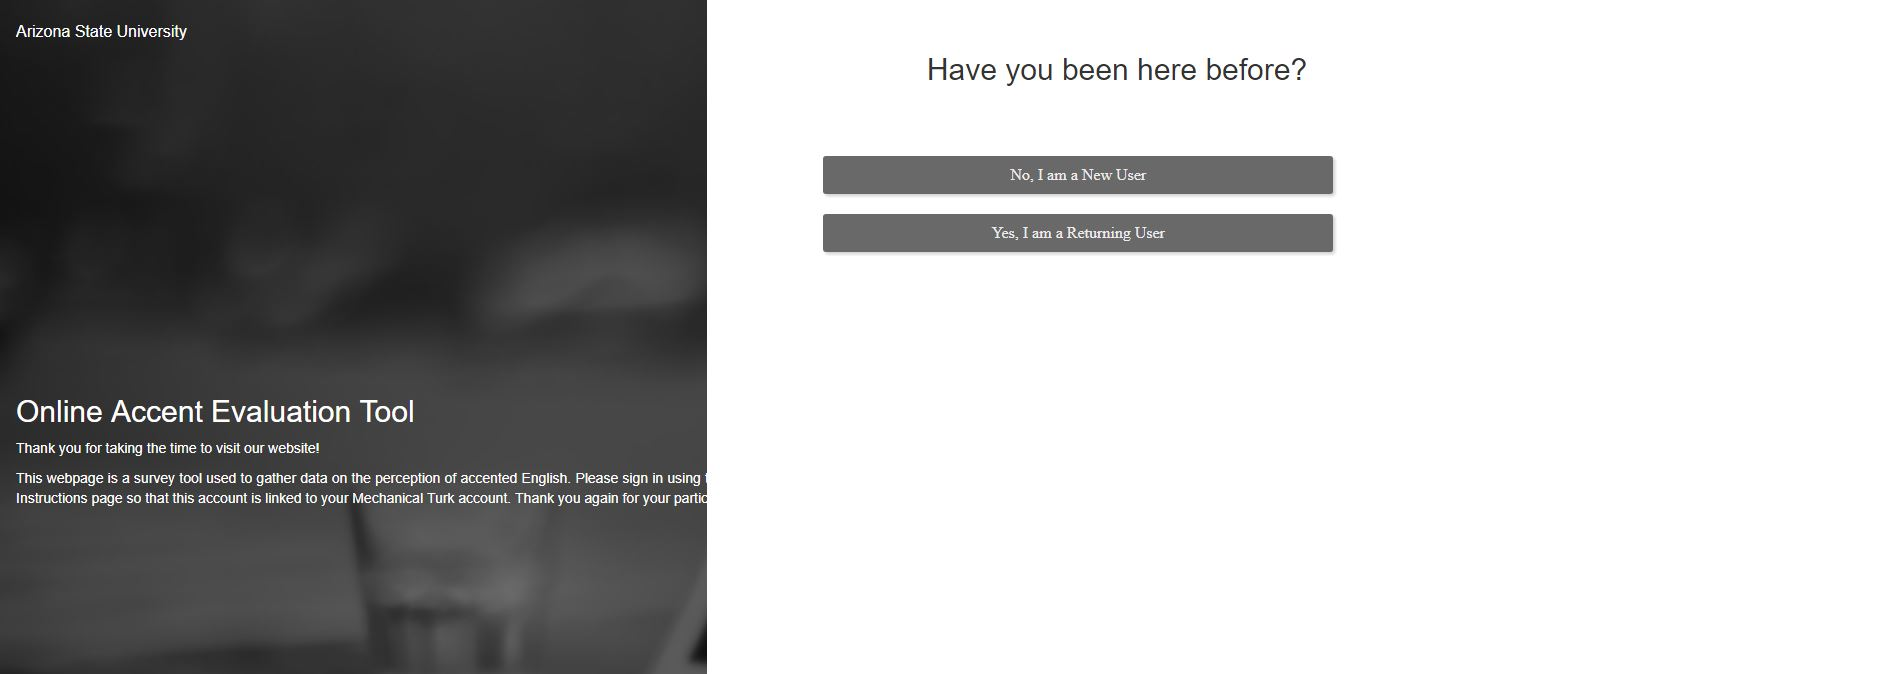
\includegraphics[width = 0.8\linewidth]{figures/webpage1.JPG}
\caption{Annotator's login page.}
\label{fig:amt_login}
\end{figure}

\begin{figure}[t]
\centering
\captionsetup{justification=centering}
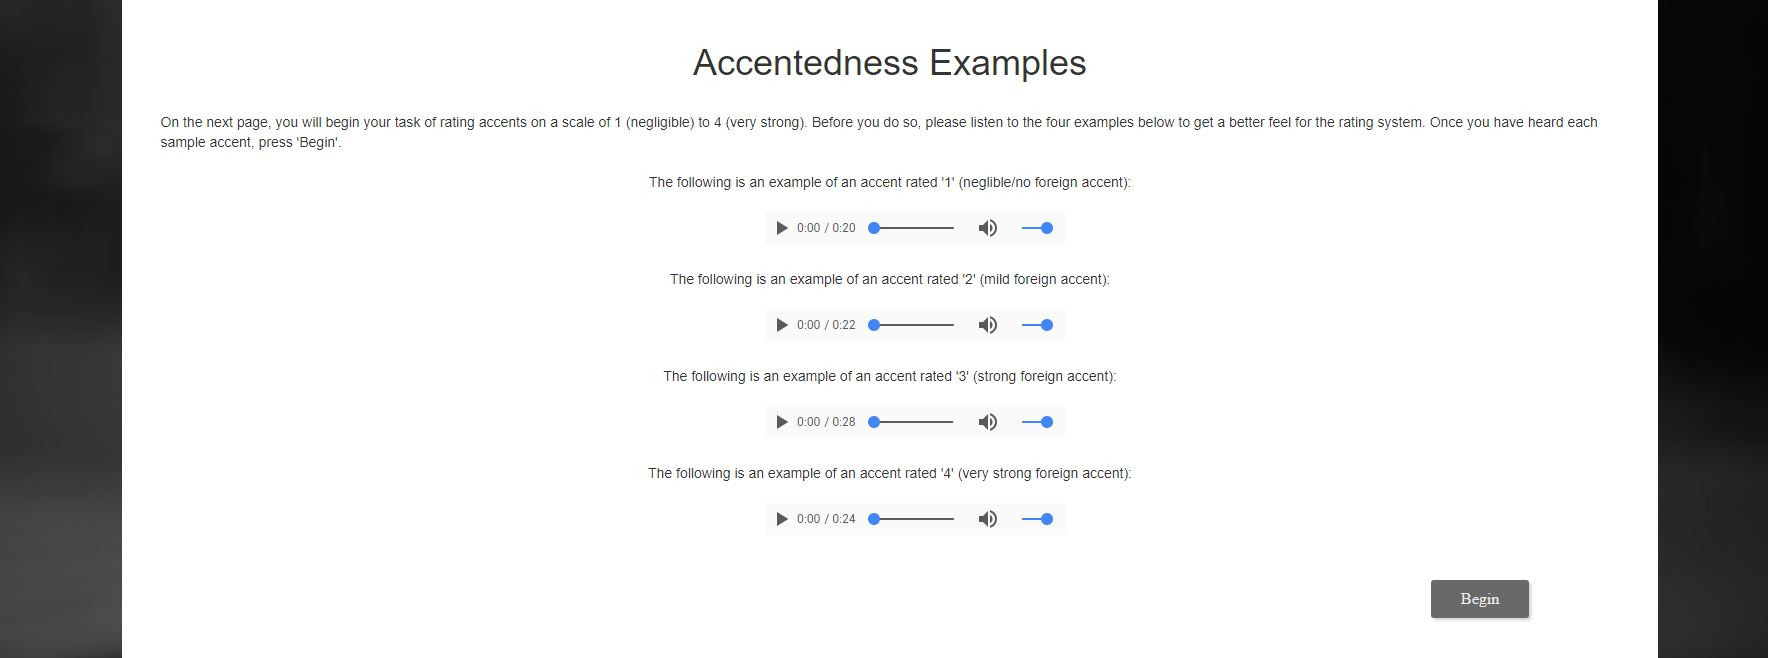
\includegraphics[width = 0.8\linewidth]{figures/webpage2.JPG}
\caption{Example accented speech recordings with groundtruth accentedness scores.}
\label{fig:amt_example}
\end{figure}

\begin{figure}[t]
\centering
\captionsetup{justification=centering}
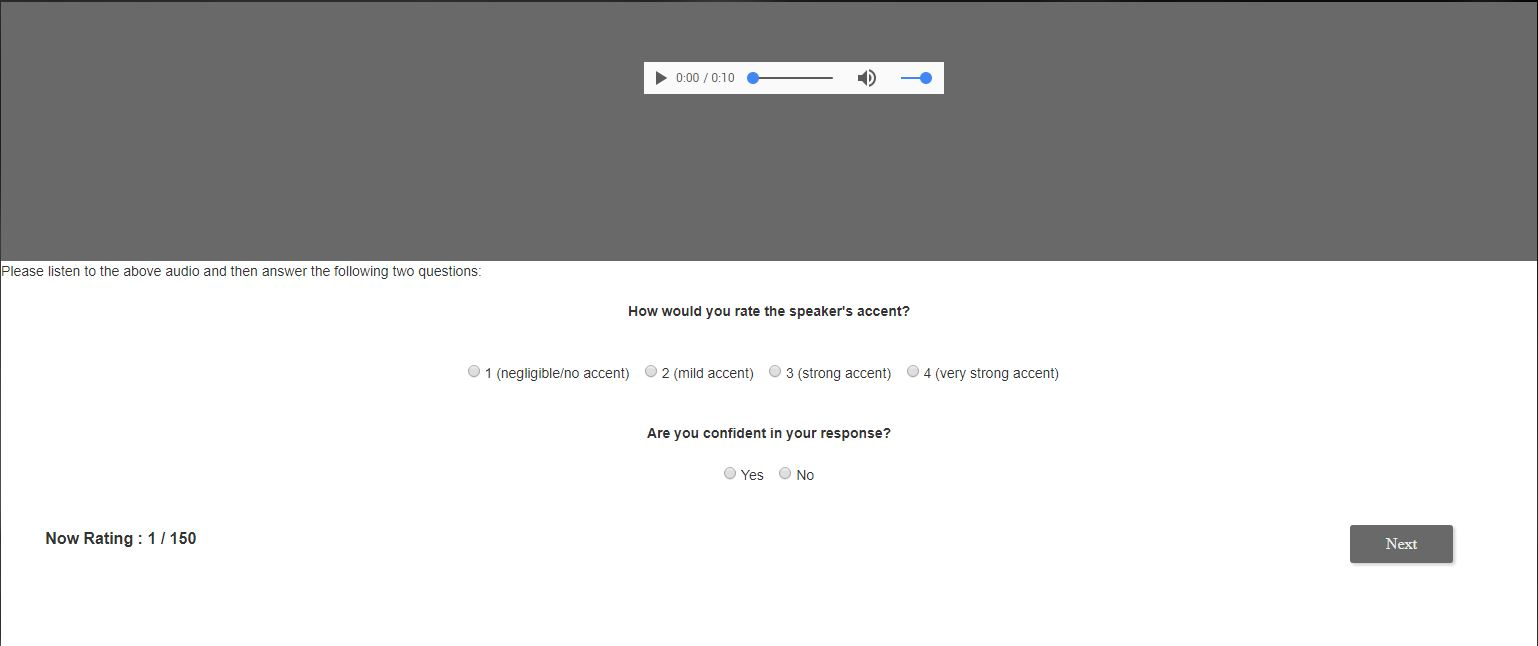
\includegraphics[width = 0.8\linewidth]{figures/webpage3.JPG}
\caption{How speech samples are presented to the annotators in listening task.}
\label{fig:amt_listen}
\end{figure}

Finally, 13 evaluators finished all the listening tasks. The average ratings of all 13 evaluators are taken as the final accentedness rating of each speaker; other studies have used the average of 10 AMT non-expert annotations in other natural language tasks \cite{snow2008cheap}. The pairwise average inter-rater correlation coefficients are shown in figure \ref{fig:pairwise_corr} for each rater, which is calculated by taking the average of the correlation coefficients of the current worker's ratings with other worker's ratings. The average inter-rater correlation coefficients (calculated as the average of all annotators' correlation with other annotators) is 0.73, which is higher enough to prove the consistency of the ratings from 13 evaluators. In figure \ref{fig0}, the histograms of the collected ratings across four different foreign languages are presented. It can be found that Mandarin speakers have the strongest accent while German speakers have the mildest accent. This is consistent with expectations considering the phonological similarity between German and English as opposed to other 3 languages. The low mean and lack of strongly-accented speakers in the German and French database also means that the variances of the accentedness ratings for these language are relatively low. This poses a challenge in the statistical modeling, which will be further examined in later chapters.

\begin{figure}[t]
\centering
\captionsetup{justification=centering}
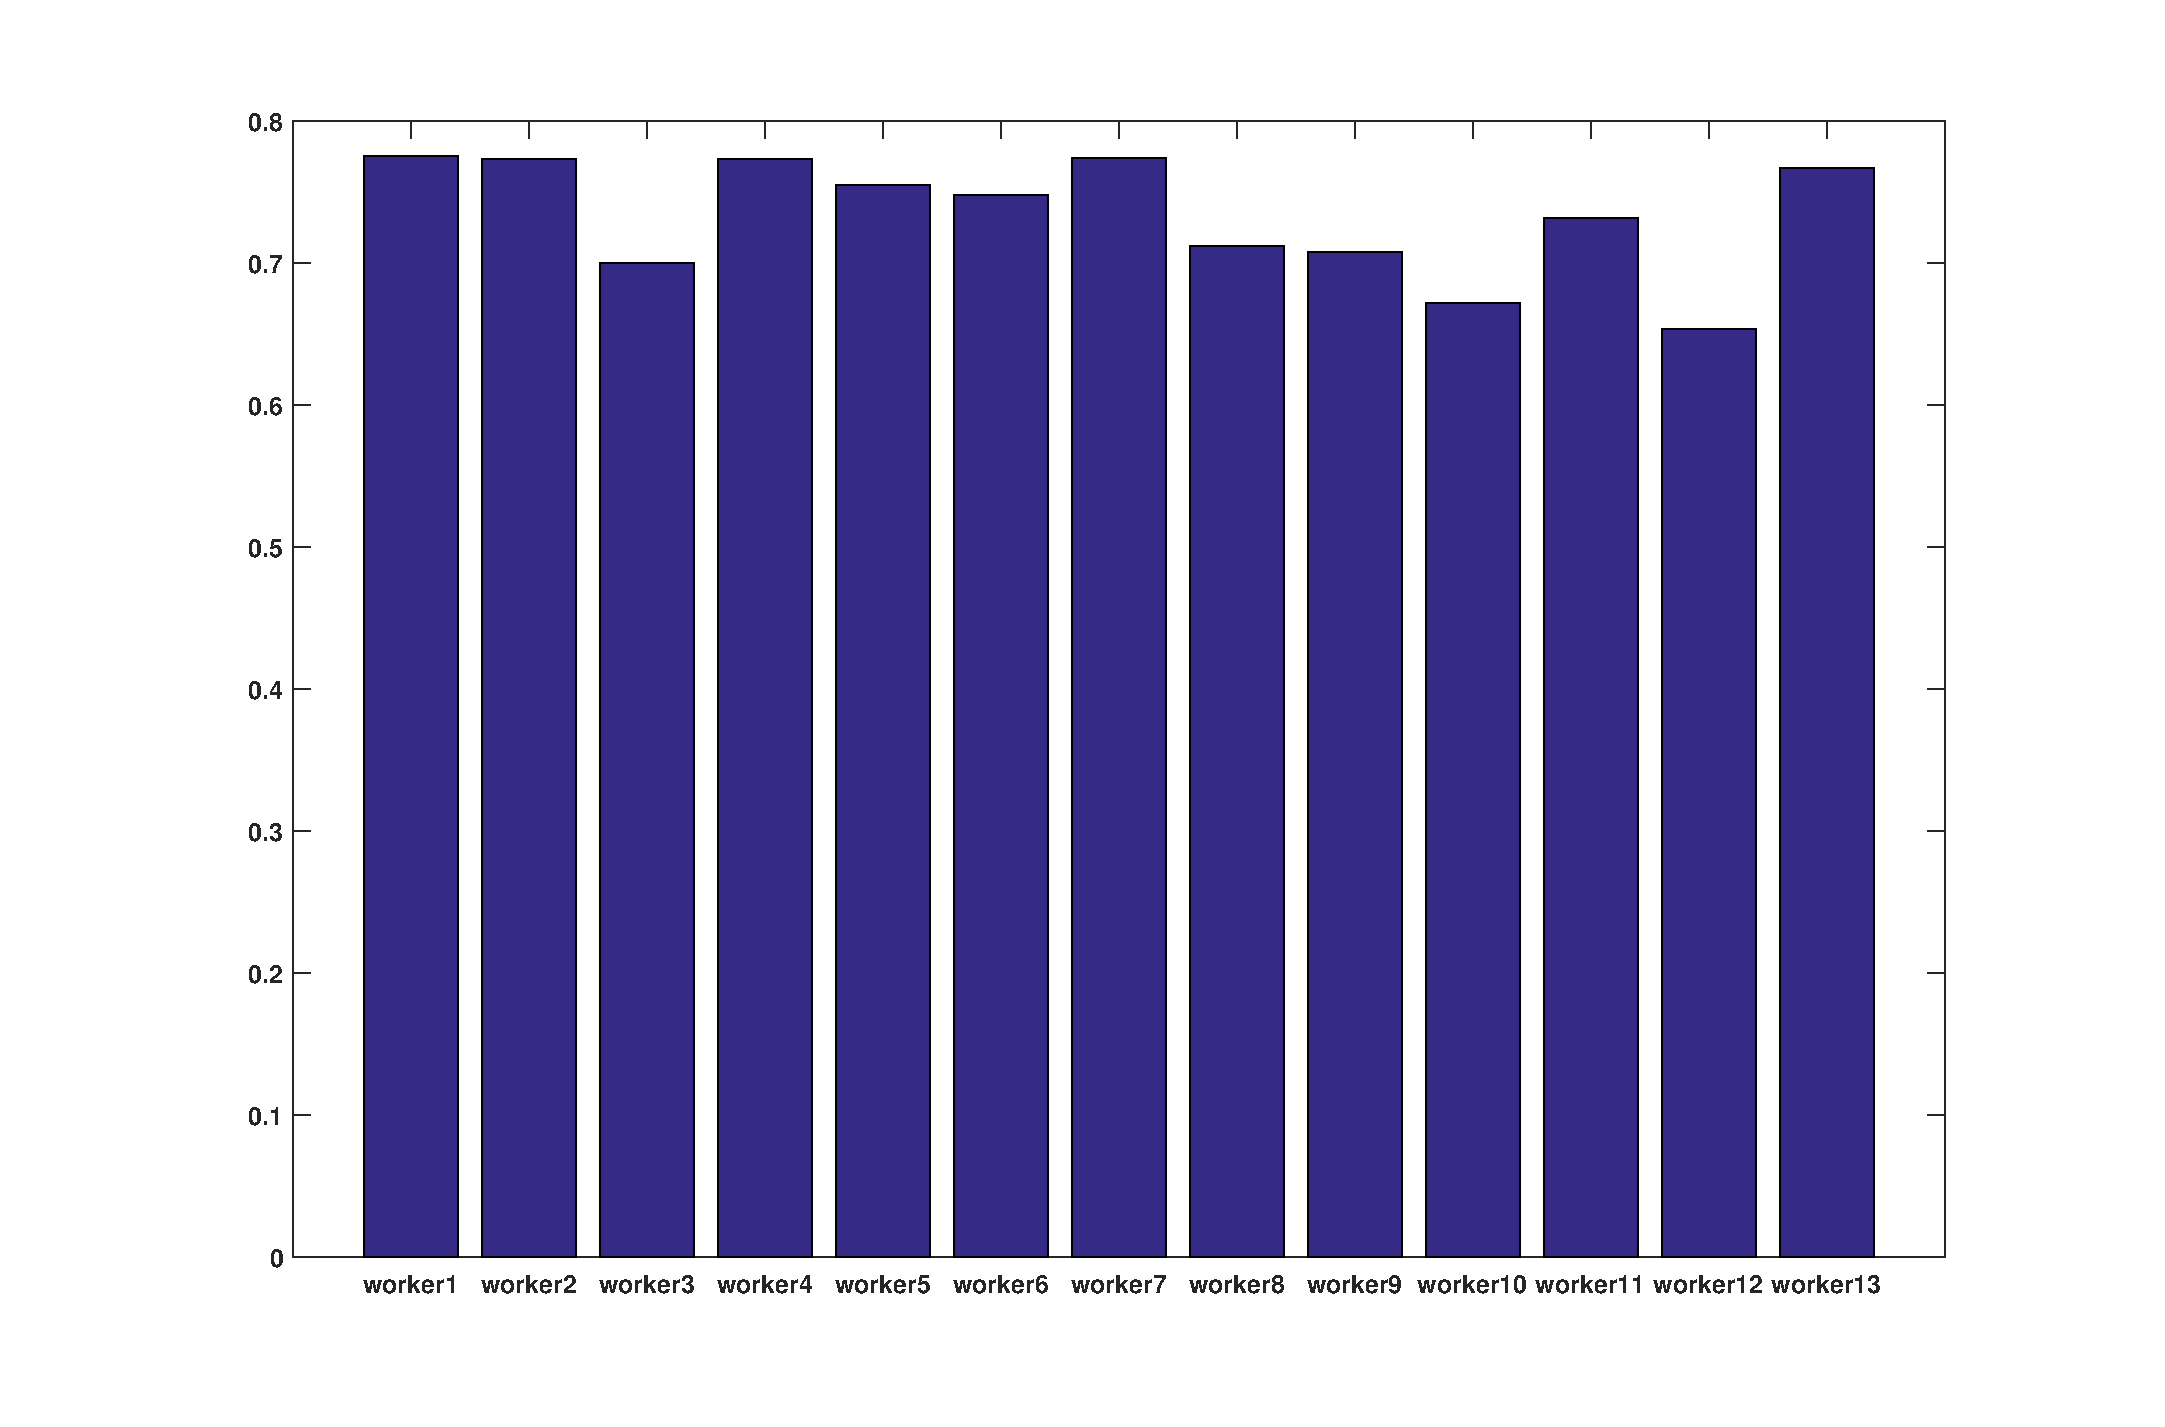
\includegraphics[width = 0.8\linewidth]{figures/mean_pairwise_correlation_without_work4.eps}
\caption{Pairwise average correlation correlation coefficients for each worker.}
\label{fig:pairwise_corr}
\end{figure}

\begin{figure}[h]
        \begin{minipage}[t]{0.5\linewidth}
        \centering
            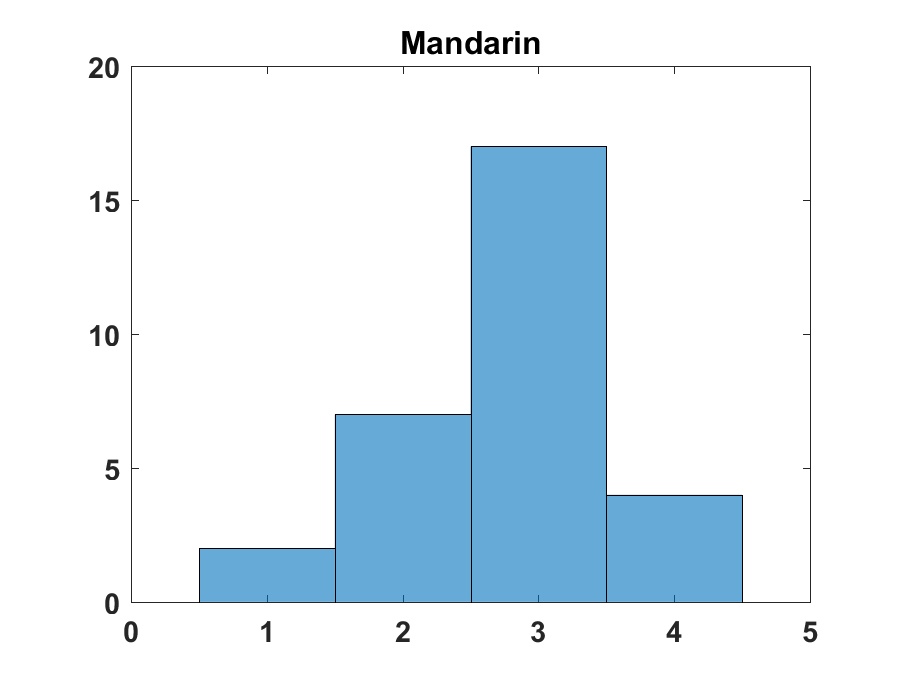
\includegraphics[width=3in]{figures/Mandarin_hist.eps}
        \end{minipage}%
        \begin{minipage}[t]{0.5\linewidth}
        \centering
            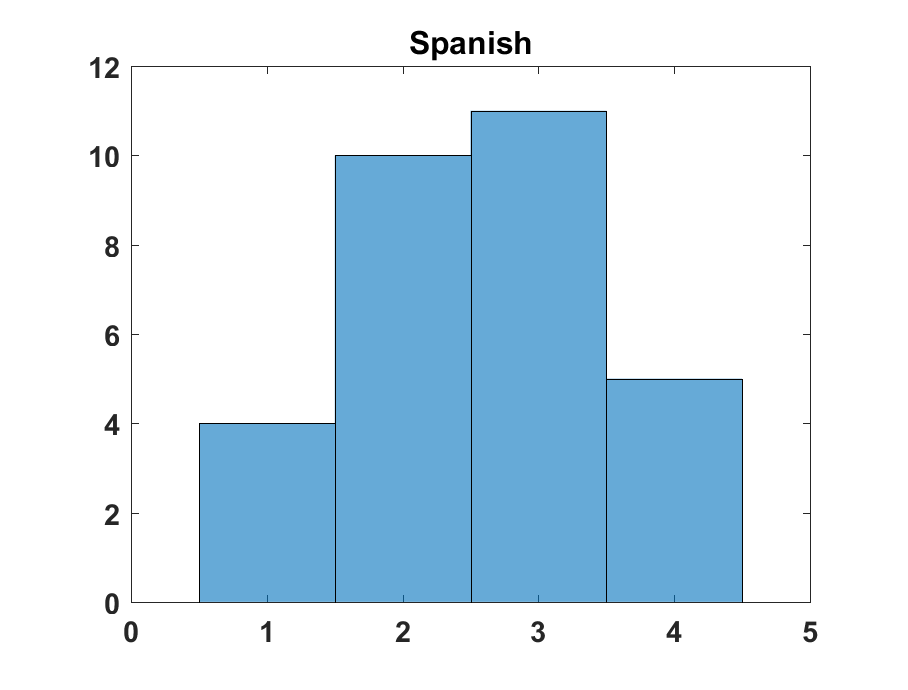
\includegraphics[width=3in]{figures/Spanish_hist.eps}
        \end{minipage}%
        \\
        \begin{minipage}[t]{0.5\linewidth}
        \centering
            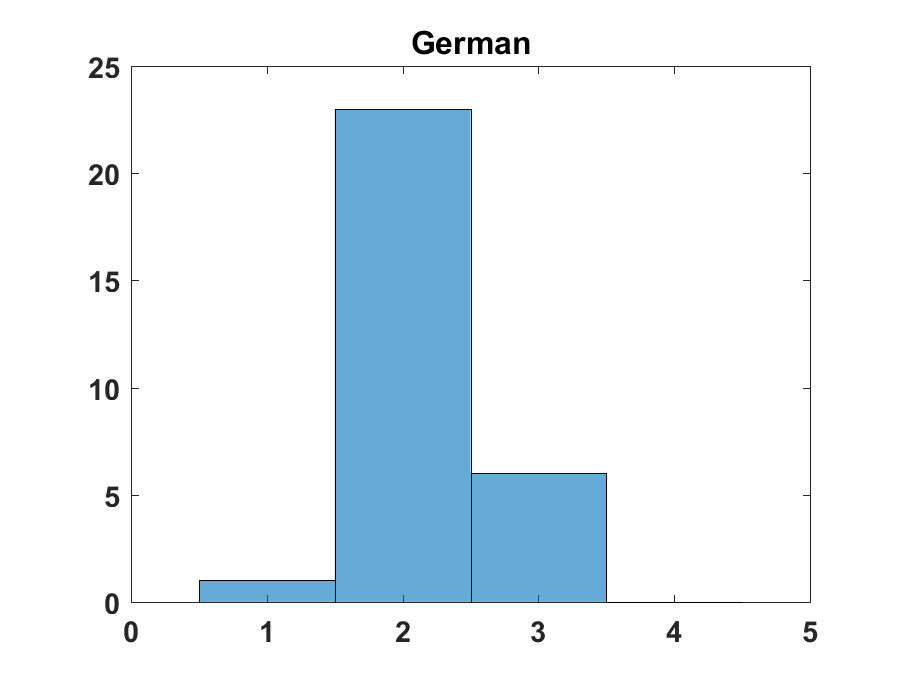
\includegraphics[width=3in]{figures/German_hist.eps}
        \end{minipage}%
        \begin{minipage}[t]{0.5\linewidth}
        \centering
            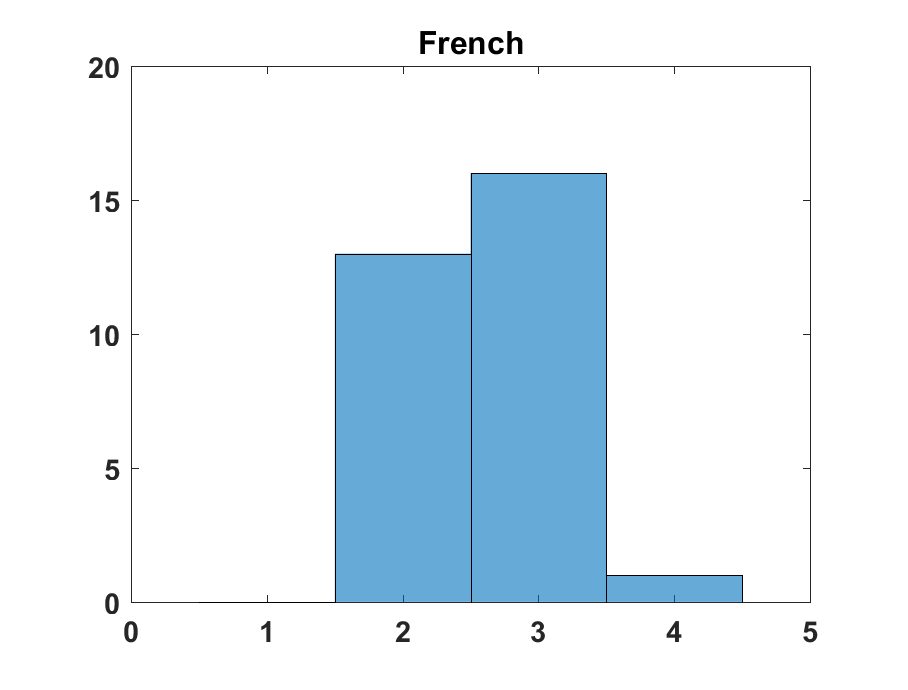
\includegraphics[width=3in]{figures/French_hist.eps}
        \end{minipage}%
        \caption{Histograms of accentedness scores of different L1s.}
        \centering
        \label{fig0}
     \end{figure}

\section{Acoustic analysis}

With the accentedness score for each speakers in the accented speech dataset collected, next step is to extract measurements from the acoustic signal to represent the foreign accent of each speaker. As mentioned in chapter \ref{introduction}, this study will analyze acoustic measurements in two subspaces: one is characterized by phonetic measurements and the other is characterized by prosodic measurements. Thus, the acoustic analysis here is also done in the two subspaces. Specifically, pronunciation scores of phonemes (including vowels and consonants) and syllables are calculated as representation of the phonetic subspace. The pronunciation scores are calculated based on previous studies on phoneme-level goodness of pronunciation \citep{witt2000phone}, which relies on a already-trained automatic speech recognition (ASR) system on native L2 speech. Prosodic measurements are calculated based on the studies by \cite{ramus1999correlates,grabe2002durational}. In this dissertation, more prosodic measurements are included compared by the previous studies as in \citep{lai2013applying}. Furthermore, the main contribution of this study is to investigate the relationship between L1 related acoustic measurements and accentedness score. To calculate L1 related acoustic measurements, corpus of different L1s (German, French, Spanish and Mandarin in this study) are also needed. The remaining part of this section will first briefly review the basic concepts of an ASR system. Then, L1 corpus used in this study will be introduced. Finally, acoustic feature extraction scheme for both phonetic and prosodic information will be presented.

\subsection{A brief introduction to ASR}

\begin{figure}[t]
\centering
\captionsetup{justification=centering}
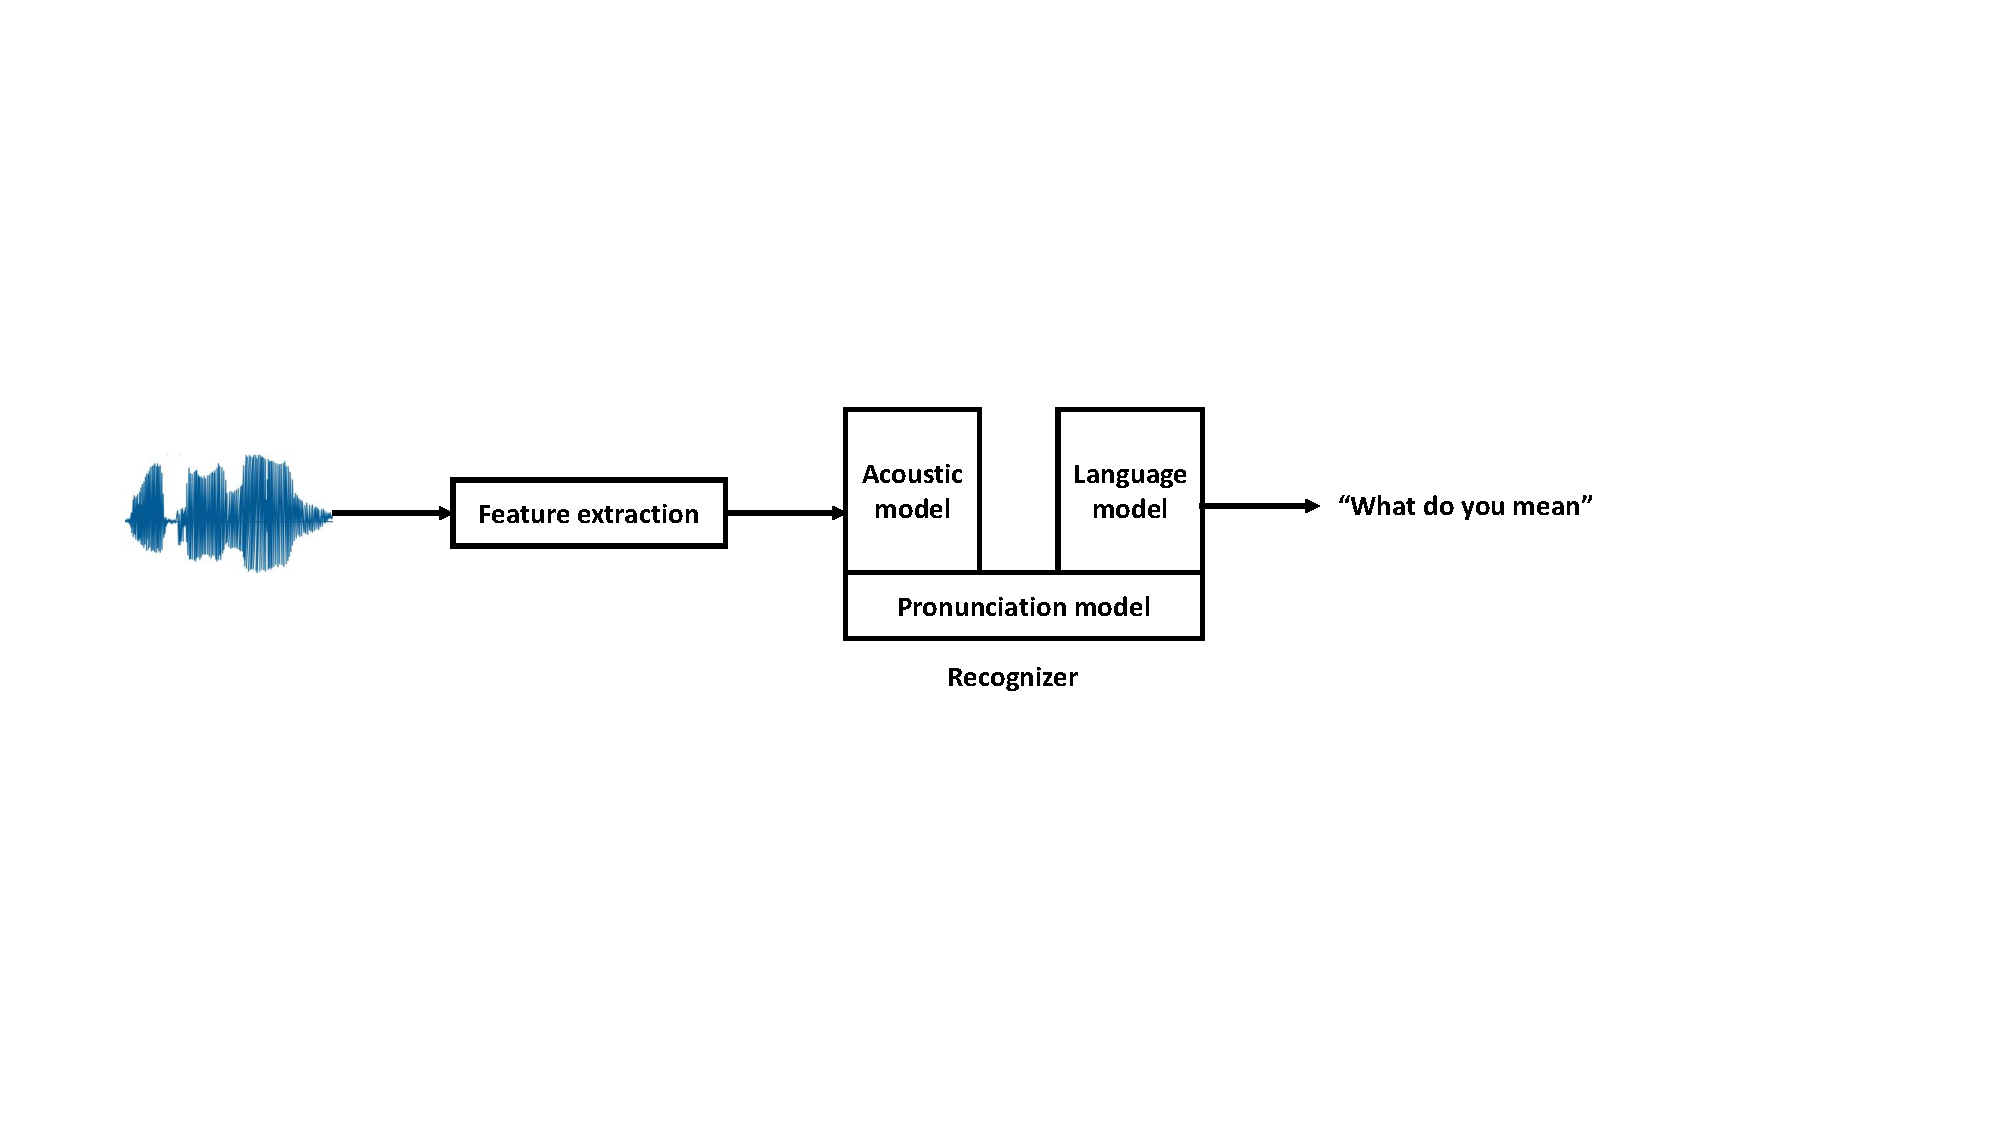
\includegraphics[width = 1.0\linewidth]{figures/ASR_diagram.pdf}
\caption{Diagram of a typical ASR system. The content of the speech signal is ``what do you mean''.}
\label{fig:asr_diagram}
\end{figure}

 Basically, ASR is trying to recognize the content, i.e. what the speaker is saying, in a speech signal. It requires knowledge from different fields, including psychoacoustics and signal processing, linguistics and machine learning\footnote{Recent developments on ASR mainly focus on the machine learning part.}. A simplified diagram of an ASR system is shown in figure \ref{fig:asr_diagram}. The input waveform is first analyzed within short windows (e.g. 25ms), also referred as frames, based on the assumption that spectral information is stationary in a short window. This process is done frame by frame. Then, a feature (usually based on Discrete Fourier Transformation) vector is calculated to represent the spectral information in each frame. The 1-dimensional time domain signal is then converted to a 2-dimensional time-frequency representation. Since phonemes can be discriminated based on spectral information in acoustic signal, this feature vector is believed to carry information of the identity of phoneme.

 \begin{figure}[t]
\centering
\captionsetup{justification=centering}
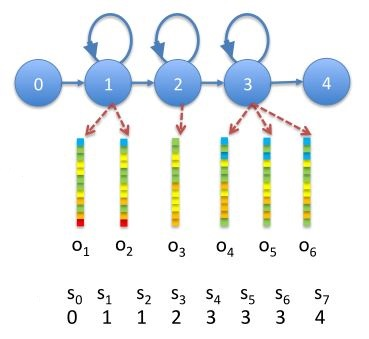
\includegraphics[width = 0.4\linewidth]{figures/HMM_state.JPG}
\caption{How an HMM aligns input feature vectors with output state sequence.}
\label{fig:hmm_diagram}
\end{figure}

 The feature vectors of a sentence is sent to recognizer, which includes three parts: acoustic model, language model and pronunciation model. Acoustic model builds the relationship between feature representation and phonemes. A sequence machine learning model called Hidden Markov Model (HMM) is employed to learn the dynamic transition from one phoneme to another based on observed feature vectors in each short window by aligning each frame with a state of HMM model. The reason to use HMM is that the number of frames is different from the number of phonemes in a sentence. There must be a way to correspond each frame to a sub-phoneme unit, which is called a state in HMM. Each HMM models one phonemes and the final acoustic model will have many HMMs. As the HMM shown in figure \ref{fig:hmm_diagram}, input feature vectors $o_1$ to $o_6$ are mapped to a state sequence $s_1$ to $s_6$, each of which corresponds to state IDs $\{1,2,3\}$. At each frame, it either moves to the next state or stay at the current state. State 0 and 4 are the entrance and exit state of the HMM, which allows transition from a previous phoneme and exit from the current phoneme. Most of the time, a triphone([k-ae+t], [k] is to the left of [ae] and [t] is to the right) instead of a single phone([ae]) is used as the basic modeling unit of an HMM for the reason that triphone can better model the coarticulation among neighboring phonemes and improve model capability. In summarization, the acoustic model converts a sequence of feature vectors to a sequence of HMM states, and then to phoneme sequence according to the mapping between HMM states to phonemes.

 The language model is for converting phoneme sequence output by acoustic model to feasible word sequences which complies with human usage of words. The pronunciation model involves in this process: it gives the phoneme sequence of each single word in a language. In a nutshell, pronunciation model is just the lexicon(or dictionary) of a language in most of the time. Pronunciation model will also be used to convert word sequences in transcription to phoneme sequences during training of the acoustic mode. There is another term commonly seen in ASR field: forced-alignment. It refers to the process to find the start and end time of a phoneme, word or even sentence in a speech signal given the transcription. This can be achieved using acoustic model and pronunciation model. A lot of studies in computational linguistics use forced-alignment to avoid locating phonemes and words in a speech signal by hand. Practically, Kaldi toolkit \citep{povey2011kaldi} is the most commonly used software to build an ASR system and it has been well accepted by academia and industry.

\subsection{Native speech corpus}
In this study, both the L2 and L1s acoustic models are needed to extract pronunciation score based phonetic features. To build the L2 acoustic model (English for this study), the LibriSpeech corpus \citep{panayotov2015librispeech} was used and the corresponding training scripts\footnote{https://github.com/kaldi-asr/kaldi/tree/master/egs/librispeech/s5} in the Kaldi toolkit. The final acoustic model is a triphone model trained with Gaussian Mixture Model-Hidden Markov Model on 960 hours of speech data. The feature input is a 39-dimensional second order Mel-Frequency Cepstral Coefficient (MFCC) with utterance-level cepstral mean variance normalization and Linear Discriminant Analysis transformation.

For Mandarin, the publicly accessible AIShell Mandarin Speech corpus (approximately 150 hours training data) \citep{bu2017aishell} and the corresponding Kaldi scripts\footnote{https://github.com/kaldi-asr/kaldi/tree/master/egs/aishell/s5} are used. A pronunciation dictionary is included with the dataset. For the remaining three languages (Spanish, French and German), there are no well organized publicly available data. We use data from the Voxforge project and download the speech corpora for French ($\approx$ 30 hours), German ($\approx$ 50 hours) and Spanish ($\approx$ 50 hours). Kaldi scripts\footnote{https://github.com/kaldi-asr/kaldi/tree/master/egs/voxforge/s5} for the Voxforge The dictionary for these three languages are from the CMU Sphinx (Download available\footnote{https://sourceforge.net/projects/cmusphinx/files/Acoustic\%20 \\ \hspace*{4mm} and\%20Language\%20Models/}). Feature types and structures of acoustic models for the four languages are the same as those used in the English acoustic model.

\subsection{Pronunciation score based phonetic feature extraction}
\label{sec:segmental}

\subsubsection{Features based on the L2 acoustic model}
\label{sec:L2_measure}

Motivated by the work by \cite{witt2000phone}, the goodness of pronunciation for each phoneme is calculated in the accented speech. To do this, the accented speech is first force-aligned at the phoneme-level using the L2 acoustic model to provide the start and end frame indices of each phoneme. The pronunciation score ($PS_{\mathrm{L2}}$) of the target phoneme $p$ after alignment is defined as
\begin{equation}
\label{gop}
\begin{aligned}
PS_{\mathrm{L2}}(p) &= \log(P(p|\mathbf{O}^{p}))/\left | \mathbf{O}^{p} \right | \\
      &= \log \left [ \frac{P(\mathbf{O}^{p}|p)P(p)}{\sum_{q\in \mathit{Q}} P(\mathbf{O}^{q}|q)P(q)} \right ] /\left | \mathbf{O}^{p} \right |,
\end{aligned}
\end{equation}
where $\mathbf{O}^{p}$ is the feature matrix of phoneme $p$, $\left |\mathbf{O}^{p}\right |$ is the number of frames of phoneme $p$ after alignment, and $\mathit{Q}$ is the set of all phonemes. If we assume equal priors for all phonemes, we approximate the denominator in Eq. \ref{gop} with max operator,

\begin{equation}
\label{gop2}
PS_{\mathrm{L2}}(p) = \log \left [ \frac{P(\mathbf{O}^{p}|p)}{\max_{q\in \mathit{Q}} P(\mathbf{O}^{q}|q)} \right ] /\left | \mathbf{O}^{p} \right |.
\end{equation}

The conditional likelihood of each phoneme (given the speech frames of the corresponding aligned segment) can be calculated by decoding the sequence of speech features using the L2 acoustic model. It is clear that if the most likely phoneme returned by the acoustic model is the same as the target phoneme $p$, then $PS_{\mathrm{L2}}(p)=0$; otherwise, this value will be negative. The interpretation is that the closer $PS_{\mathrm{L2}}(p)$ is to zero, the closer the pronunciation of phoneme $p$ is to that of native speakers.

\subsubsection{L1 acoustic model based measurements}
\label{sec:L1_measure}

In contrast to the $PS_{\mathrm{L2}}$ score, there is no transcript to measure the pronunciation of the phonemes in L1. We define a new way to calculate the pronunciation score with the L1 acoustic model which quantifies how close the pronunciation of a phoneme in L2 is to a specific phoneme in L1. The forced-alignment calculated with the L2 acoustic model is used here. The speech frames are first decoded with the L1 acoustic model and find the state path with the highest likelihood. In the path, the corresponding phonemes of each HMM state are recorded and the phoneme with the highest occurrence is considered as the most likely L1 phoneme for a given speech segment. Then, the pronunciation score is calculated as

\begin{equation}
\label{l1gop}
PS_{\mathrm{L1}}(p) = \left [ \sum_{t \in T_p} \log \frac{ \sum_{s \in S_p}P(o_t|s)}  { \sum_{s \in S}P(o_t|s)} \right ] /\left | T_p \right |,
\end{equation}
where $o_t$ is the feature vector for frame $t$ and $p$ is the phoneme with the highest occurrences in the best decoding path of the current segment. $T_p$ is the set of frames where each frame corresponds to an HMM state of phoneme $p$. $S_p$ is the set of HMM states that belong to phoneme $p$ and $S$ is the set of all HMM states. $PS_{\mathrm{L1}}(p)$ essentially quantifies the confidence of the L1 acoustic model that phoneme $p$ was produced for a speech segment. With equation \ref{l1gop}, a pronunciation score based on the L1 acoustic model can be calculated for each phoneme segment in the original alignment. The implementations of both feature sets are available on Github\footnote{https://github.com/tbright17/kaldi-dnn-ali-gop}.

\subsubsection{Sentence-level integration}

Previous introduced feature extraction methods will output both $PS_{\mathrm{L2}}$ and $PS_{\mathrm{L1}}$ on phoneme level. However, accented speech of each speaker is a sentence. Thus, a sentence-level integration method is proposed to convert phoneme-level pronunciation scores to a sentence-level feature vector. Specifically, after phoneme-level features $PS_{\mathrm{L2}}(p)$ and $PS_{\mathrm{L1}}(p)$, are extracted, \a sentence-level feature extraction scheme was used to convert phoneme-level measurements to a feature vector with a fixed dimension for each utterance. The pronunciation features for vowels, consonants and syllables are first grouped together and four statistics for each of these three phonetic categories are then calculated: for both $PS_{\mathrm{L2}}(p)$ and $PS_{\mathrm{L1}}(p)$, the minimum, mean, standard deviation and mean-normalized standard deviation (standard deviation divided by mean) of phoneme-level pronunciation measurements of vowels, consonants and syllables in each utterance are calculated (implementation available\footnote{https://github.com/tbright17/accent-feat}). This results in a total of 12 utterance-level features for the acoustic model of each language, and a total of 24 utterance-level features combining both pronunciation information from L1 and L2 acoustic models.

\subsection{Prosodic feature extraction}
\label{sec:supraseg}

To represent speech prosody, durational rhythmic measurements of phonemes and syllables are adopted as the studies by \cite{ramus1999correlates,grabe2002durational}. Specifically, an extended speech rhythmic feature set proposed in \citep{lai2013applying} are employed in this study. First, the same forced-alignment results achieved in previous section is reused here to get the start and end time of each phoneme. Then, the following measurements are calculated:
\begin{enumerate}
\item Mean, standard deviation and mean-normalizd standard deviation (standard deviation divided by mean) of durations of vowels, consonants and syllables.
\item Duration proportion of vowels, consonants and syllables, calculated as the total length of vowels, consonants and syllables divided by the length of the sentence.
\item Raw Pairwise Variability Index (rPVI) of durations of vowels, consonants and syllables, calculated as:
    \begin{equation}
    \label{eq:rPIV}
    rPVI= \sum_{k=1}^{m-1} |d_k-d_{k+1}|/(m-1),
    \end{equation}
    where $d_k$ is the duration of $k$th phoneme or syllable and $m$ is the total number of phonemes or syllables in a sentence.
\item Normalized Pairwise Variability Index (nPVI) of durations of vowels, consonants and syllables, calculated as:
    \begin{equation}
    \label{eq:nPIV}
    nPVI= \sum_{k=1}^{m-1} |\frac{d_k-d_{k+1}}{(d_k + d_{k+1})/2}|/(m-1),
    \end{equation}
    where the notations are the same as in equation \ref{eq:rPIV}.
\end{enumerate}

Finally, a 18-dimensional feature vector can be extracted from each speech signal. In this study, this rhythmic feature extraction scheme is applied to both L1 speech, L2 speech and accented speech to do contrastive analysis between accented speech and L1 and between L2 speech and accented speech. For the four foreign languages, 1000 sentences with more than 40 phonemes are randomly selected from the corresponding native speech corpus. For native English, those measurements are directly calculated on the 30 native American English sentences from SAA.

\section{Procedure}

 \begin{figure}[t]
\centering
\captionsetup{justification=centering}
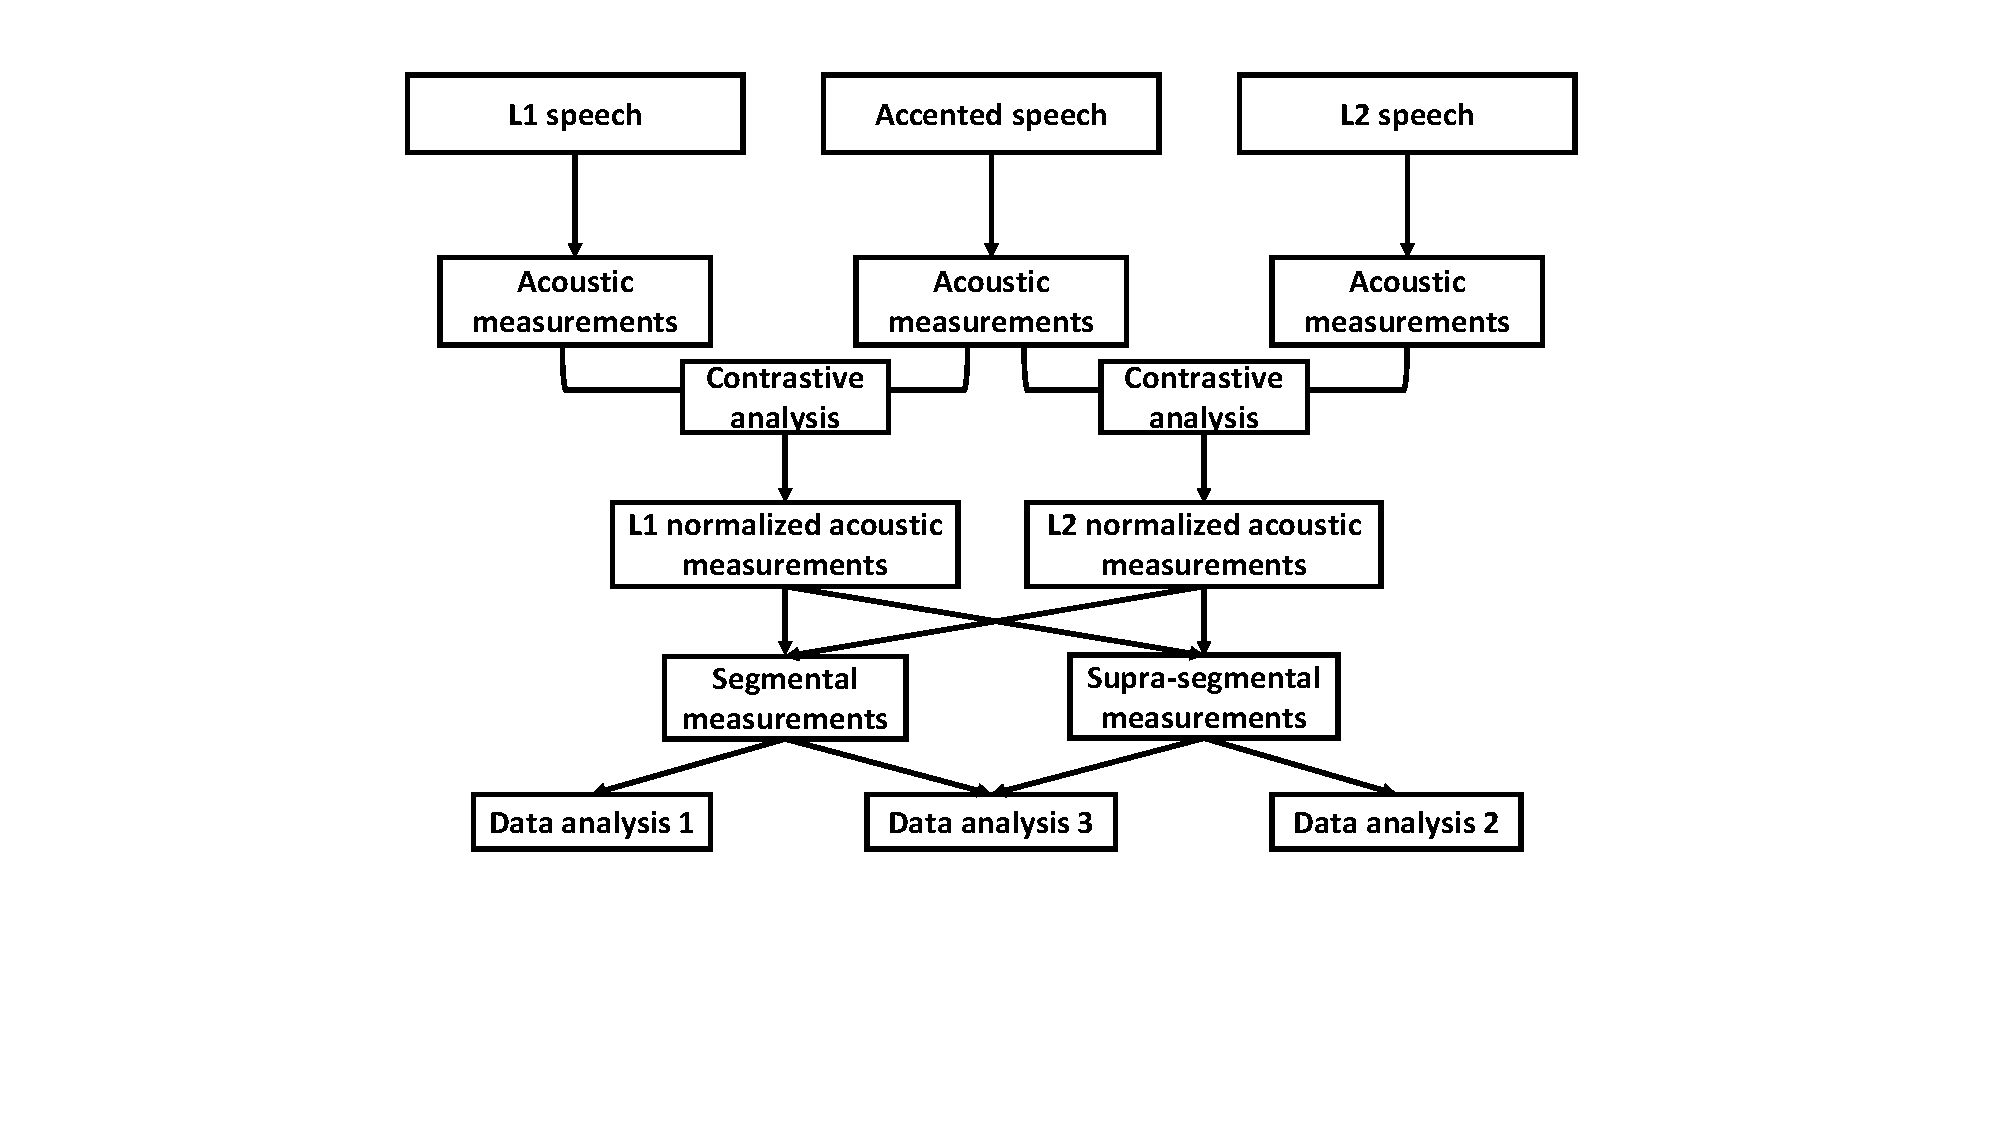
\includegraphics[width = 0.8\linewidth]{figures/method_diagram.pdf}
\caption{Diagram of the methodology used in this study.}
\label{fig:method_diagram}
\end{figure}

The diagram of the methodology used in this study is shown in figure \ref{fig:method_diagram}. After extracting acoustic measurements from native L1 speech, accented speech and native L2 speech, contrastive analysis, the goal of which is to quantify the difference between two sets of features is applied on the L1-accented pair and L2-accented pair. Then two sets of features can be obtained: the L2 normalized acoustic measurements represent how close the phonological properties in accented speech is to native L2 speech; the L1 normalized acoustic measurements represent how close the phonological properties in accented speech is to native L1 speech. The segmental feature extraction scheme in section \ref{sec:segmental} directly output the L1 and L2 normalized acoustic measurements because the input of the method is accented speech and L1 or L2 acoustic model and the output is already contrastive. In contrast, contrastive analysis needs to be done for the supra-segmental feature extraction method in section \ref{sec:supraseg}. Both these two sets of features can be further categorized into segmental measurements and supra-segmental measurements. The first data analysis, which will be introduced in chapter \ref{l1_seg}, will investigate the effect of L1 phonological properties on the phonetic system of accented speech.  The second data analysis, which will be introduced in chapter \ref{l1_supraseg}, will investigate the effect of L1 phonological properties on the prosodic system of accented speech. The third data analysis, which will be introduced in chapter \ref{both_l1_l2}, will investigate the effect of L1 phonological properties on both the phonetic and prosodic systems of accented speech and propose a new computational model to do automatic accentedness evaluation. The data analysis methods used in this study are mainly the correlational analysis, which examines how the acoustic measurements and accentedness score are correlated, and multiple regression analysis, which examines how well the combination of multiple acoustic measurements can predict the accentedness score. The data analysis procedure involves feature preprocessing, feature selection and mode regularization, which will be introduced in detail in later chapters. 